\documentclass[12pt, french]{article}

\usepackage{fancyhdr, fancybox, lastpage, makecell}
\usepackage[most]{tcolorbox}
\usepackage[a4paper, margin={0.3in, .75in}]{geometry}
\usepackage{wrapfig}
\pagestyle{fancy}
\renewcommand\headrulewidth{1pt}
\renewcommand\footrulewidth{1pt}
\fancyhf{}
\rhead{ \em{Zakaria Haouzan}}
\lhead[C]{\em{Filière Tronc Commun Scientifique }}
\chead[C]{}
\rfoot[C]{}
\lfoot[R]{}
\cfoot[]{\em{Page \thepage / \pageref{LastPage}}}


\newtcolorbox{Box2}[2][]{
                lower separated=false,
                colback=white,
colframe=white!20!black,fonttitle=\bfseries,
colbacktitle=white!30!gray,
coltitle=black,
enhanced,
attach boxed title to top left={yshift=-0.1in,xshift=0.15in},
title=#2,#1}


\begin{document}
\begin{center}
   \shadowbox {\bf{ Soutien en physique et chimie}}
\end{center}


%%_________________________Exercice 5 : _________________________Exercice
\begin{Box2}{Exercice 1 :(Extrait de l'examen 2016 – Casablanca Settat) }
	On réalise une chronophotographie d’une voiture
qui roule sur le sol suivant une trajectoire
rectiligne, au cours des différentes étapes de son
mouvement. la durée qui sépare la prise de deux
images successives est t=1,6s.

\begin{center}
	%\begin{wrapfigure}[lineheight]{position}{width}
    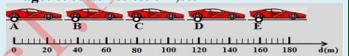
\includegraphics[width=0.5\textwidth ]{./img/voiture.png}
  \end{center}

  \begin{enumerate}
	  \item Calculer , en m/s et Km/h , la vitesse moyenne
de la voiture entre A et C.
\item Donner , en justifiant la réponse , la nature du
mouvement de la voiture.
\item Le conducteur de la voiture a aperçu un danger
sur la route et a essayé de s'arrêter, il n'a pu
appuyer sur les freins qu’après 1,5s.
\begin{enumerate}
	\item Déterminer,en mètre,la distance dR parcourue
par la voiture pendant le temps de réaction (1,5s),
si la vitesse de la voiture est de 25 m/s.
\item Dans les conditions de circulation de cette
	voiture, la distance de freinage est calculée par la relation $d_F(m) = \frac{v^2}{15,4}$ , où V est la vitesse de la
voiture au début du freinage en m/s. Calculer la
distance de freinage dF et déduire la distance
d'arrêt $d_A$.
\end{enumerate}
  \end{enumerate}

\end{Box2}



%%_________________________Exercice 6 : _________________________Exercice


\begin{Box2}{Exercice 2 : (Extrait de l'examen 2016 – Fes Meknes) }

	\begin{wrapfigure}[5]{r}{0.275\textwidth}
\begin{center}
	\vspace{-0.8cm}

    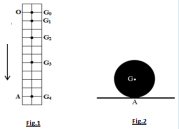
\includegraphics[width=0.3\textwidth]{./img/boulehomog.png}
  \end{center}

	\end{wrapfigure}
On lance une boule homogène S depuis la position O et
elle tombe vers la position A, et on enregistre les
positions consécutives du point G de la boule
(G0, G1, G2, G3 ,.) Comme indique la figure 1.

La durée qui sépare deux emplacements consécutifs est
constante et égale à t = 0,1s, et la distance OA = 1m.
\begin{enumerate}
	\item Déterminer la nature de la trajectoire du point G
pendant que la balle tombe.
\item Déterminer la nature du mouvement de la balle en
justifiant la réponse.
\item Calculer la durée T pendant laquelle la balle tombe
de la position O à la position A.
\item Calculer la vitesse moyenne Vm du point G entre les
positions O et A.
\item La balle S se trouve en position A au-dessus d'une
table horizontale et maintient son équilibre
\begin{enumerate}
	\item Faire le bilan exercées sur la balle (S)
	\item Classer ces forces en forces de contact et en
forces à distance.
\item Donner les caractéristiques de la force $\vec{R}$  exercée
par la table sur la boule sachant que son intensité
est égale à 4N.
\item Représenter sur (la balle) , en choisissant
comme échelle la force de contact exercée
sur la balle.
\end{enumerate}
\end{enumerate}

\end{Box2}


%%_________________________Exercice 7 : _________________________Exercice

\begin{Box2}{Exercice 3 : Ressort }
	\begin{wrapfigure}[5]{r}{0.268\textwidth}
	%\vspace{-1cm}
    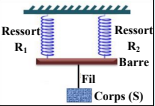
\includegraphics[width=0.3\textwidth]{./img/Ressort.png}
  \caption{}
	\end{wrapfigure}
Réalisons l’expérience suivante :
\begin{enumerate}
	\item Faire le bilan des actions
mécaniques exercées sur la
barre.
\item Classer ces fores en : 
	\begin{enumerate}
		\item Forces de contact et forces à distance.
		\item Forces localisées et forces réparties.

	\end{enumerate}
\item Représenter, en choisissant une échelle
convenable, les forces de contact exercées sur la
barre sachant qu’elles ont la même intensité qui
égale à 3N.
\end{enumerate}
\end{Box2}


%%_________________________Exercice ! :"_________________________Exercice
   \begin{Box2}{Exercice 4 :La loi d’ohm} 
	   \begin{enumerate}
   \item Quelle intensité traverse un conducteur ohmique de résistance $400\Omega$ s’il est soumis à
une tension de 40 V?
\item Un conducteur ohmique est traversé par un courant de 10 mA quand il est soumis à
une tension de 20 V. Quelle est la valeur de la résistance?
\item Un conducteur ohmique de résistance de $1000\Omega$ est parcouru par un courant de
220 mA. A quelle tension est-il soumis?
\end{enumerate}
   \end{Box2}


%%_________________________Exercice ! :"_________________________Exercice
   \begin{Box2}{Exercice 5 :La La puissance électrique} 
   
	   Un restaurant est contient des appareils électriques suivants :
	   \begin{itemize}
		   \item Un four électrique (220V – 1200W)
		   \item Télévision écran plat (220V – 400W)
		   \item Chauffe-eau (220V – 1800W)
	   \end{itemize}
	   \begin{enumerate}
		   \item Que signifier les valeurs enregistrées sur le four électrique (220V – 1200W) ?
		   \item Calculer l’intensité de courant électrique I traversant le four électrique pendant
son fonctionnement normal.
\item Calculer la résistance électrique (R) de ce four électrique.
\item On fonctionne tous ces appareils en même temps,  Calculer la puissance électrique totale (Pt) consommée par ces appareils.
	   \end{enumerate}

   \end{Box2}

   \begin{Box2}{Exercice 6 :Les atomes et les ions }
	   L’ion Dichromate est constitue de deux atomes de chrome (Cr) et 7 atomes d’oxygène
	   sachant de la charge total de cet ion est $-3,2.10^{-19}C$ et la charge de son cortège
	   électronique est $-1,696.10^{-17}C$
	   \begin{enumerate}
		   \item Donner le type de L’ion
		   \item Donner sa formule
		   \item Déduire le nombre des électrons et déduire le numéro atomique
		   \item Calculer alors le numéro atomique de l’atome de chrome (Cr) sachant que Z(O) = 8
		   \item Remplissez le tableau suivant\\ 
			   \begin{center}
\begin{tabular}{ |c|c|c|c|c|c| }
	\hline
	\makecell{  Symbole \\de l’atome} & \makecell{Numéro\\ atomique} & \makecell{Symbole\\de l’ion} & \makecell{La charge \\du noyau\\de l’atome} & \makecell{La charge\\des électrons\\de l’ion} &\makecell{La charge\\globale\\de l’ion} \\\hline 
 Cl & 17 & $Cl^-$ &.... & .... & ....  \\  \hline
 .... & .... & .... &+8e & .... & -2e  \\  \hline
 .... & 7 & .... &.... & .... & -3e  \\  \hline
\end{tabular}
\end{center}
	   \end{enumerate}
   \end{Box2}

   \begin{Box2}{Exercice 7 : }
	   On fait brûler de l'Aluminium dan un bocal de 700 ml contenant du dioxy-
gène. Avant la combustion la masse de l'Aluminium et de 4g lorsque tout le

dioxygène a été consommé,la combustion cesse et il reste 2,9g de
l'Aluminium.
\begin{enumerate}
	\item Écrivez l'équation- bilan équilibrée de la combustion de l'Aluminium.
	\item Calculez la masse de l'Aluminium qui a brûlé.
	\item Calculez la masse de dioxygène consommé, sachant que la masse de 1 litre
de dioxygène est de 1,3g .
\item Calculez la masse de dioxyde d'Aluminium obtenu.
\end{enumerate}
   \end{Box2}
   \begin{Box2}{Exercice 8 : }
complétez les réactions d'oxydations suivantes :

$...Al+ ...O_2 \rightarrow ...Al_2O_3$ \hspace{2cm} $....+ ...O_2 \rightarrow ...CuO$

$...Fe+ ...O_2 \rightarrow ...Fe_3O_4$ \hspace{2cm} $....+ ...O_2 \rightarrow ...ZnO$

   \end{Box2}

   \begin{Box2}{Exercice 9:}
Les masses volumiques du cuivre et du zinc sont respectivement $8920 kg/m^3$
et $7140 kg/m^3$.
   \begin{enumerate}
	   \item Comment calculer la masse volumique du laiton contenant 90\% de cuivre et 10\% de zinc.
	   \item Si on note x le pourcentage de zinc dans le laiton, exprimer la masse
volumique du laiton en fonction de x sachant que le laiton n'est
constitué que de cuivre et de zinc.
   \end{enumerate}
\end{Box2}

\end{document}
